\chapter{Test of Latex functions}\label{app:test-of-latex-functions}

\section{Math Functions}
\textbf{How to include math functions:}
\begin{align}
    E & = mc^2                                 \\
    m & = \frac{m_0}{\sqrt{1-\frac{v^2}{c^2}}}
\end{align}

\section{Listing elements and Tables}
%Für Aufzählungen stehen unter LaTeX die Umgebungen itemize, description und enumerate zur Verfügung. Innerhalb der Aufzählung wird jedes neue Element mit dem Befehl \item eingeleitet. Selbstverständlich können Aufzählungen auch ineinandergeschachtelt werden.

\textbf{Enumerate}
\begin{enumerate}
    \item First
    \item Second
    \item Third
\end{enumerate}

\textbf{Listing}
\begin{description}
    \item{First}
    \item{Second}
    \item{Third}
\end{description}

\textbf{Unordered Listing}
\begin{itemize}
    \item{Info}
    \item{Point}
    \item{Listing}
\end{itemize}

\subsection{Besondere Aufzählungen}

%Mit \usepackage{paralist} lässt sich die Art der Aufzählung ändern:
%
%\begin{compactenum}[(i)] %führt zu (i), (ii), (iii), (iv), ...
%\begin{compactenum}[(I)] %führt zu (I), (II), (III), (IV), ...
%\begin{compactenum}[a)] %führt zu a), b), c), d), ...

\begin{compactenum}[(i)]
    \item{Erster Punkt}
    \item{Zweiter Punkt}
    \item{Dritter Punkt}
\end{compactenum}

\begin{compactenum}[(I)]
    \item{Erster Punkt}
    \item{Zweiter Punkt}
    \item{Dritter Punkt}
\end{compactenum}

\begin{compactenum}[(a)]
    \item{Erster Punkt}
    \item{Zweiter Punkt}
    \item{Dritter Punkt}
\end{compactenum}

\subsection{Verschachtelte Aufzählungen}

%~\par sorgt dafür das, dass vorangestellte Item wie so eine kleine Überschrift verwendet wird. Löscht es einfach mal, dann seht ihr was passiert!
\begin{description}
    \item[Nummerierte Aufzählung]~\par
    \begin{enumerate}
        \item Weitere Aufzählung
              \begin{enumerate}
                  \item erstens.
                  \item zweitens.
              \end{enumerate}
        \item Toter Punkt
    \end{enumerate}

    \item[Nichtnummerierte Aufzählung]~\par
    \begin{itemize}
        \item Unteraufzählung
              \begin{itemize}
                  \item erstens.
                  \item zweitens.
              \end{itemize}
        \item der andere Punkt.
    \end{itemize}
\end{description}

\newpage

\section{Tabellen}
%Alles über Tabellen könnt Ihr hier nochmal nachlesen: http://en.wikibooks.org/wiki/LaTeX/Tables (Auf Englisch)


%c 	Zentrierter Text
%l 	linksbündiger Text
%r 	rechtsbündiger Text

\begin{table}[!htb]
    \begin{tabular}{ l c r }
        1 & 2 & 3 \\
        4 & 5 & 6 \\
        7 & 8 & 9 \\
    \end{tabular}
    \caption{Tabelle 1}
    \label{first_table} % "tab:first_table" to keep organizing tidy
\end{table}




\begin{tabular}{ l | c || r }
    1 & 2 & 3 \\
    4 & 5 & 6 \\
    7 & 8 & 9 \\
\end{tabular}



\begin{tabular}{ l | c || r }
    \hline
    1 & 2 & 3 \\
    4 & 5 & 6 \\
    7 & 8 & 9 \\
    \hline
\end{tabular}



\begin{center}
    \begin{tabular}{ l | c || r }
        \hline
        1 & 2 & 3 \\ \hline
        4 & 5 & 6 \\ \hline
        7 & 8 & 9 \\
        \hline
    \end{tabular}
\end{center}



\begin{tabular}{|r|l|}
    \hline
    7C0         & hexadecimal \\
    3700        & octal       \\ \cline{2-2}
    11111000000 & binary      \\
    \hline \hline
    1984        & decimal     \\
    \hline
\end{tabular}

\newpage
\subsection{Breite für Spalten festlegen}

Ohne festgelegte Breite:
\begin{center}
    \begin{tabular}{| l | l | l | l |}
        \hline
        Day       & Min Temp & Max Temp & Summary                                                      \\ \hline
        Monday    & 11C      & 22C      & A clear day with lots of sunshine.
        However, the strong breeze will bring down the temperatures.                                   \\ \hline
        Tuesday   & 9C       & 19C      & Cloudy with rain, across many northern regions. Clear spells
        across most of Scotland and Northern Ireland,
        but rain reaching the far northwest.                                                           \\ \hline
        Wednesday & 10C      & 21C      & Rain will still linger for the morning.
        Conditions will improve by early afternoon and continue
        throughout the evening.                                                                        \\
        \hline
    \end{tabular}
\end{center}

Mit festgelegter Breite:
\begin{center}
    \begin{tabular}{ | l | l | l | p{5cm} |}
        \hline
        Day       & Min Temp & Max Temp & Summary                                                      \\ \hline
        Monday    & 11C      & 22C      & A clear day with lots of sunshine.
        However, the strong breeze will bring down the temperatures.                                   \\ \hline
        Tuesday   & 9C       & 19C      & Cloudy with rain, across many northern regions. Clear spells
        across most of Scotland and Northern Ireland,
        but rain reaching the far northwest.                                                           \\ \hline
        Wednesday & 10C      & 21C      & Rain will still linger for the morning.
        Conditions will improve by early afternoon and continue
        throughout the evening.                                                                        \\
        \hline
    \end{tabular}
\end{center}

\newpage
\subsection{Legende in der Tabelle}

\begin{table}[htb]
    \begin{tabular}{|r|l|}
        \hline
        7C0         & hexadecimal \\
        3700        & octal       \\ \cline{2-2}
        11111000000 & binary      \\
        \hline \hline
        1984        & decimal     \\
        \hline
    \end{tabular}
    \caption{Eine super interessante Tabelle}
    \label{tab:supertabelle}
\end{table}

\newpage

\section{Adding pictures/figures}
\begin{figure}[!htb]
    \begin{center}
        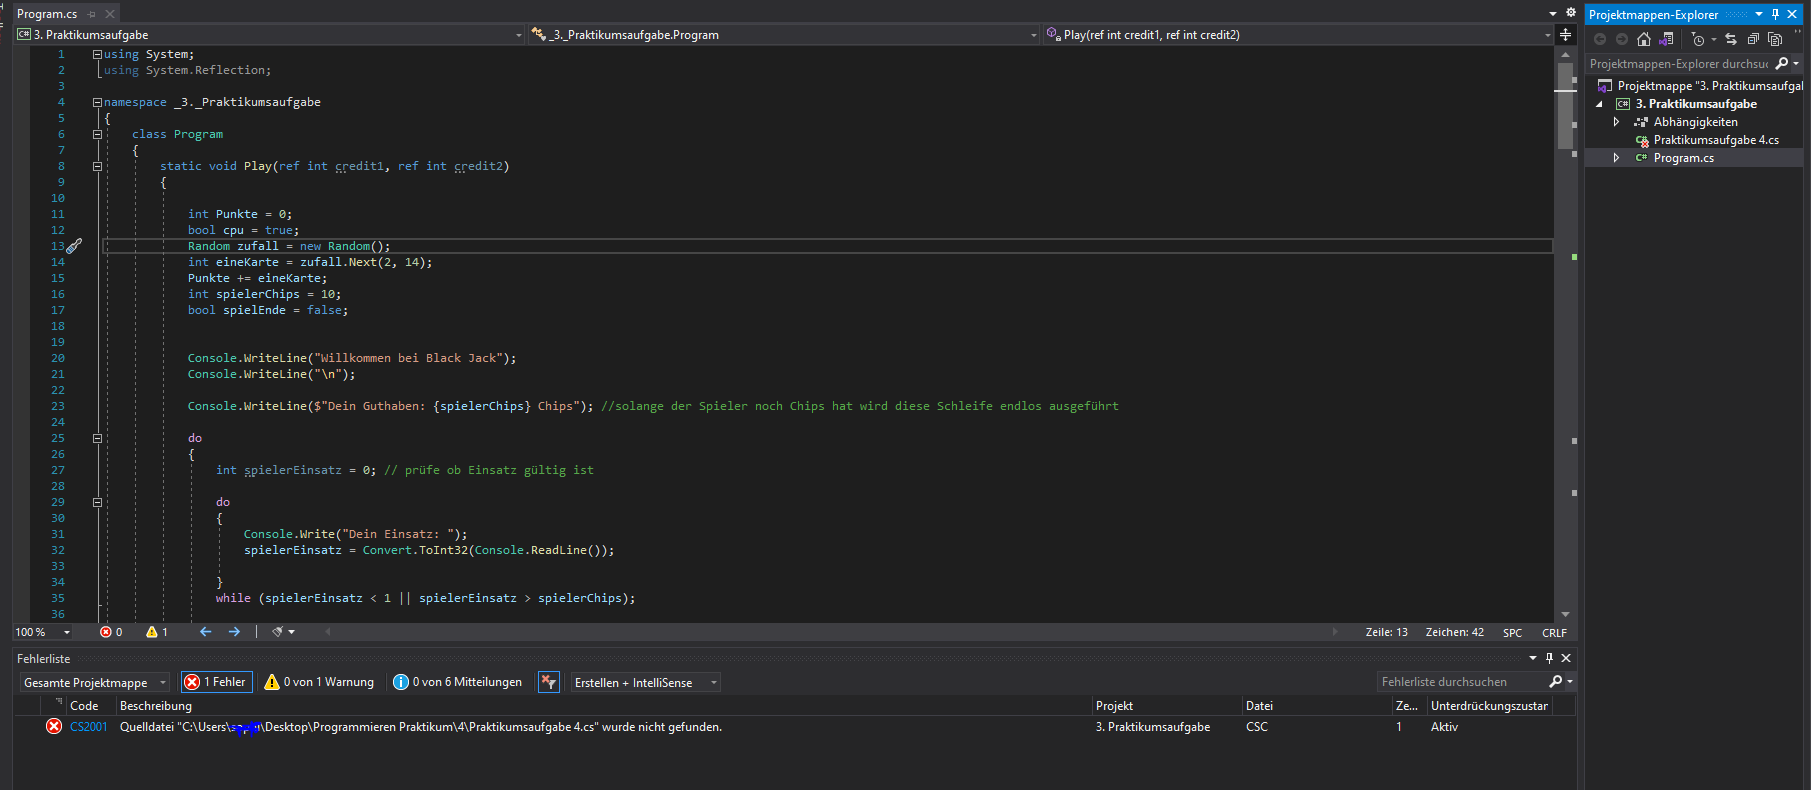
\includegraphics[width=\textwidth, keepaspectratio]{figures/example.PNG}
        \caption{Example picture test}
        \label{example_pic}
    \end{center}
\end{figure}

\section{References}

\subsection{Referencing images/figures}
Here is how you can reference you images: reference \ref{example_pic}

\subsection{Referencing sources}
Augmented Reality (AR) is a technology that enhances the real world with digital elements.
By integrating computer graphics, audio, and other sensory inputs into the physical environment, AR applications can provide the user with an enhanced and more immersive experience.
AR has gained significance in various fields in recent years, from entertainment to education and medicine.
AR offers numerous applications, particularly in the industry, where it can be used in manufacturing, maintenance, and training.
In medicine, AR can be used to visualize body parts and plan complex surgeries while detecting errors before they occur.
In education, AR technologies can help students better understand complex concepts by presenting the learned content with visual support.
Additionally, in retail, AR is increasingly being utilized to enhance the shopping experience and inform customers in innovative ways. \cite[S. 1-6]{computers11020028}

\newpage
\section{Include PDFs}


\includepdf[pages=9-10, nup=2x1]{PDF/AR_Expose} % "pages=-" for whole pdf